\documentclass[unicode,11pt,a4paper,oneside,numbers=endperiod,openany]{scrartcl}

\usepackage{minted}
\usepackage{amsmath}
\usepackage{listings}

\usepackage{ifthen}
\usepackage[utf8]{inputenc}
\usepackage{graphics}
\usepackage{graphicx}
\usepackage{hyperref}

\pagestyle{plain}
\voffset -5mm
\oddsidemargin  0mm
\evensidemargin -11mm
\marginparwidth 2cm
\marginparsep 0pt
\topmargin 0mm
\headheight 0pt
\headsep 0pt
\topskip 0pt        
\textheight 255mm
\textwidth 165mm

\newcommand{\duedate} {}
\newcommand{\setduedate}[1]{%
\renewcommand\duedate {Due date:~ #1}}
\newcommand\isassignment {false}
\newcommand{\setassignment}{\renewcommand\isassignment {true}}
\newcommand{\ifassignment}[1]{\ifthenelse{\boolean{\isassignment}}{#1}{}}
\newcommand{\ifnotassignment}[1]{\ifthenelse{\boolean{\isassignment}}{}{#1}}

\newcommand{\assignmentpolicy}{
\begin{table}[h]
\begin{center}
\scalebox{0.8} {%
\begin{tabular}{|p{0.02cm}p{16cm}|}
\hline
&\\
\multicolumn{2}{|c|}{\Large\textbf{HPC Lab for CSE 2024 ---  Submission Instructions}}\\
\multicolumn{2}{|c|}{\large\textbf{(Please, notice that following instructions are mandatory: }}\\
\multicolumn{2}{|c|}{\large\textbf{submissions that don't comply with, won't be considered)}}\\
&\\
\textbullet & Assignments must be submitted to \href{https://moodle-app2.let.ethz.ch/course/view.php?id=22516}{Moodle} (i.e. in electronic format).\\
\textbullet & Provide both executable package and sources (e.g. C/C++ files, Matlab). 
If you are using libraries, please add them in the file. Sources must be organized in directories called:\\
\multicolumn{2}{|c|}{\textit{Project\_number\_lastname\_firstname}}\\
& and  the  file must be called:\\
\multicolumn{2}{|c|}{\textit{project\_number\_lastname\_firstname.zip}}\\
\multicolumn{2}{|c|}{\textit{project\_number\_lastname\_firstname.pdf}}\\
\textbullet &  The TAs will grade your project by reviewing your project write-up, and looking at the implementation 
                 you attempted, and benchmarking your code's performance.\\

\textbullet & You are allowed to discuss all questions with anyone you like; however: (i) your submission must list anyone you discussed problems with and (ii) you must write up your submission independently.\\
\hline
\end{tabular}
}
\end{center}
\end{table}
}
\newcommand{\punkte}[1]{\hspace{1ex}\emph{\mdseries\hfill(#1~\ifcase#1{Points}\or{Points}\else{Points}\fi)}}


\newcommand\serieheader[6]{
\thispagestyle{empty}%
\begin{flushleft}

\includegraphics[width=0.4\textwidth]{ETHlogo_13}
\end{flushleft}
  \noindent%
  {\large\ignorespaces{\textbf{#1}}\hspace{\fill}\ignorespaces{ \textbf{#2}}}\\ \\%
  {\large\ignorespaces #3 \hspace{\fill}\ignorespaces #4}\\
  \noindent%
  \bigskip
  \hrule\par\bigskip\noindent%
  \bigskip {\ignorespaces {\Large{\textbf{#5}}}
  \hspace{\fill}\ignorespaces \large \ifthenelse{\boolean{\isassignment}}{\duedate}{#6}}
  \hrule\par\bigskip\noindent%  \linebreak
 }

\makeatletter
\def\enumerateMod{\ifnum \@enumdepth >3 \@toodeep\else
      \advance\@enumdepth \@ne
      \edef\@enumctr{enum\romannumeral\the\@enumdepth}\list
      {\csname label\@enumctr\endcsname}{\usecounter
        {\@enumctr}%%%? the following differs from "enumerate"
	\topsep0pt%
	\partopsep0pt%
	\itemsep0pt%
	\def\makelabel##1{\hss\llap{##1}}}\fi}
\let\endenumerateMod =\endlist
\makeatother




\usepackage{textcomp}






\begin{document}


\setassignment
\setduedate{Monday 15 April 2024, 23:59 (midnight)}

\serieheader{High-Performance Computing Lab for CSE}{2024}
{Student: Benedict Armstrong}
{Discussed with: Tristan Gabl}{Solution for Project 3}{}
\newline


\section{Implementing the linear algebra functions and the stencil
  operators}

\subsection{Linalg functions}
Implementing the eight linalg function outlined in \texttt{linalg.cpp} was relatively straighforward. Each followed a similar pattern of component wise iteration over the input array(s) and then performing the required operation. An example of the \texttt{copy} function is shown in Listing \ref{lst:linalg_copy}.

\begin{listing}[h!t]
    \begin{minted}{cpp}
    for (int i = 0; i < N; i++)
    {
        y[i] = x[i];
    }
    \end{minted}
    \caption{Linalg copy function}
    \label{lst:linalg_copy}
\end{listing}

\subsection{Stencil operators}

The next task was Implementing the stencil operator. Listing \ref{lst:stencil_operator} shows how we calculate the value for each grid cell.

\begin{listing}[h!t]
    \begin{minted}{cpp}
    f(i, j) = -(4. + alpha) * s_new(i, j) 
            + s_new(i - 1, j) + s_new(i + 1, j) 
            + s_new(i, j - 1) + s_new(i, j + 1) 
            + beta * s_new(i, j) * (1.0 - s_new(i, j)) 
            + alpha * s_old(i, j);
    \end{minted}
    \caption{Stencil operator}
    \label{lst:stencil_operator}
\end{listing}

\subsection{Plotting the results}

Finally we can plot the results with the following parameters:
\begin{itemize}
    \item $nx = ny = 128$
    \item $nt = 100$
    \item $t = 0.005$
\end{itemize}

The output of the serial version is shown in Listing \ref{lst:run_serial}.

\begin{listing}[h]
    \begin{minted}{bash}
$ ./build/main 128 100 0.005
================================================================================
                        Welcome to mini-stencil!
version   :: C++ Serial
mesh      :: 128 * 128 dx = 0.00787402
time      :: 100 time steps from 0 .. 0.005
iteration :: CG 300, Newton 50, tolerance 1e-06
================================================================================
--------------------------------------------------------------------------------
simulation took 0.15112 seconds
1514 conjugate gradient iterations, at rate of 10018.5 iters/second
300 newton iterations
--------------------------------------------------------------------------------
### 1, 128, 100, 1514, 300, 0.15112 ###
Goodbye!
    \end{minted}
    \caption{Running the serial version of the mini-app}
    \label{lst:run_serial}
\end{listing}

The results are shown in Figure \ref{fig:output_serial}.

\begin{figure}[h!t]
    \centering
    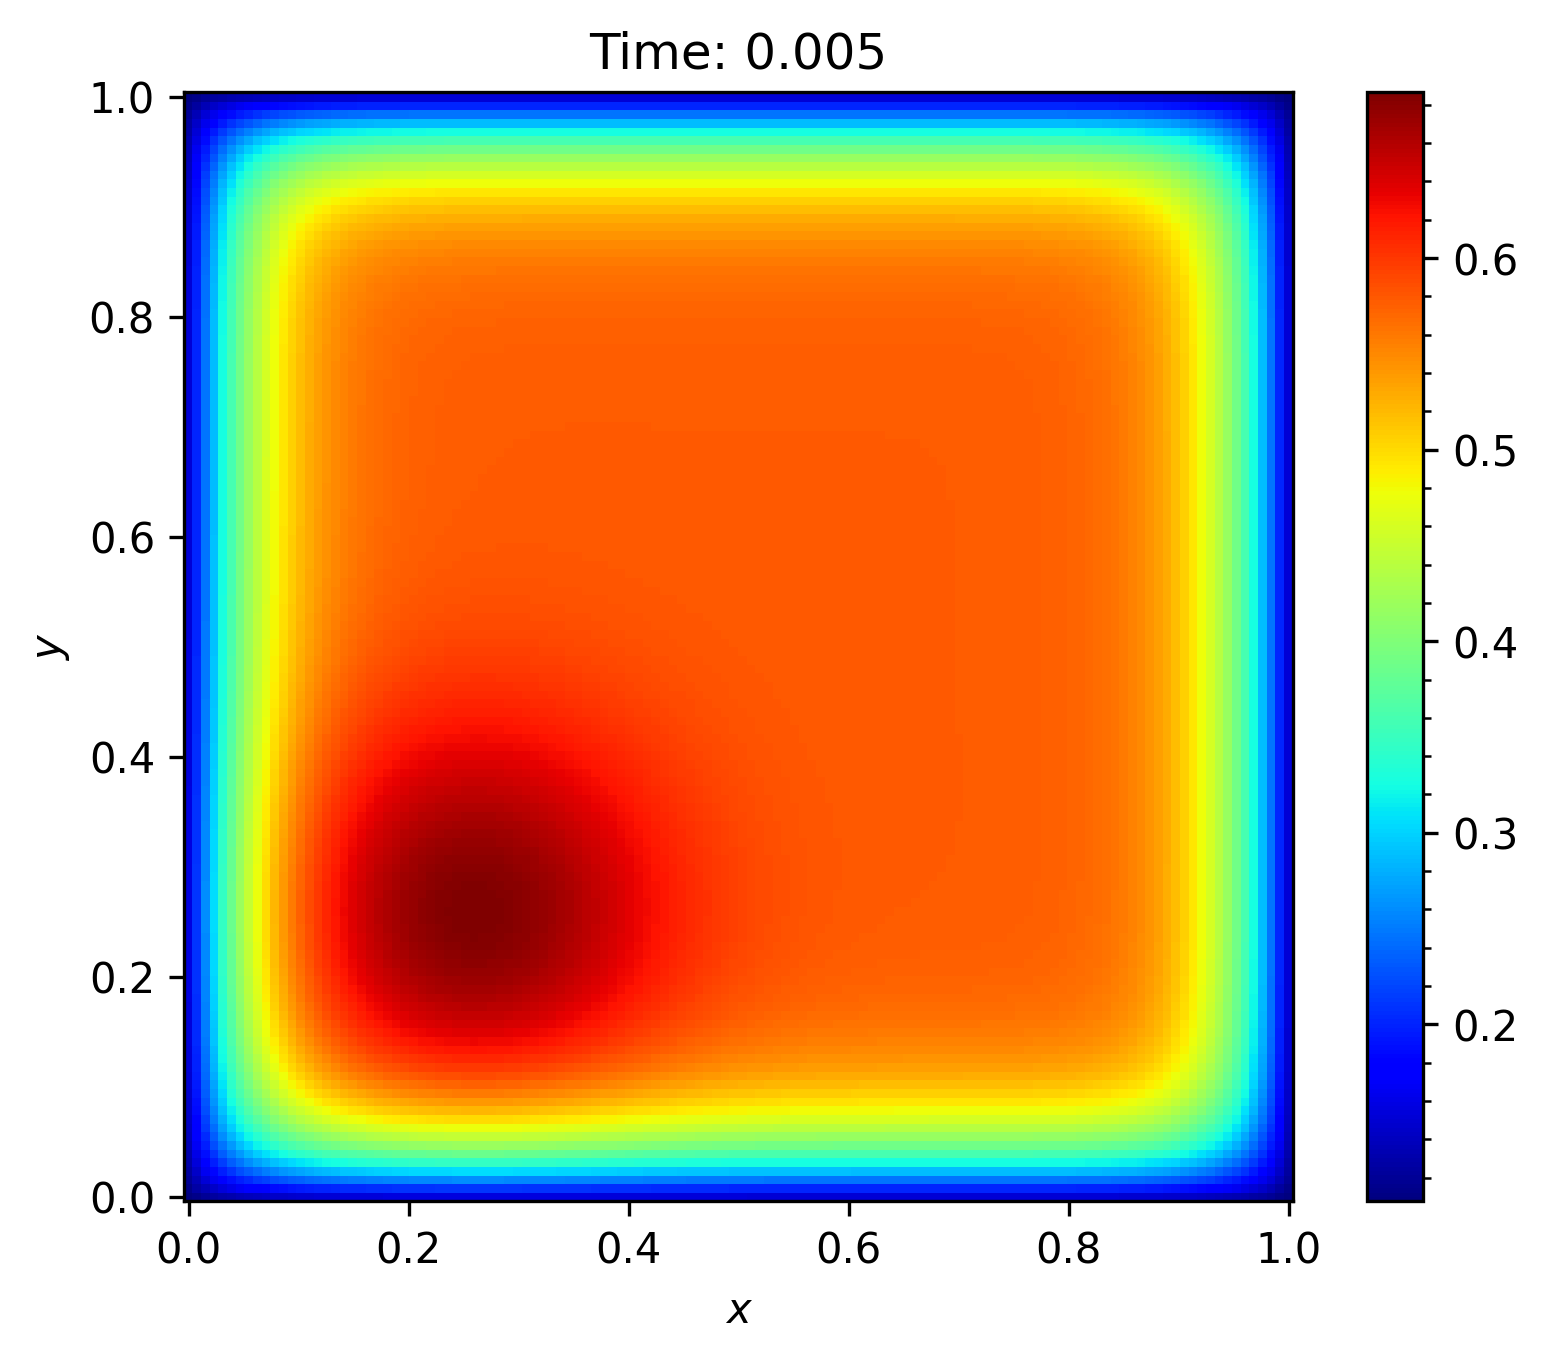
\includegraphics[width=0.5\textwidth]{plots/output_serial.png}
    \caption{Results of the nonlinear PDE mini-app}
    \label{fig:output_serial}
\end{figure}


\section{Adding OpenMP to the nonlinear PDE mini-app}

First I reconfigured the project welcome message. If \mintinline{cpp}{_OPENMP} is defined, we use \mintinline{cpp}{omp_get_max_threads()} to get the number of threads. The code welcome message is shown in Listing \ref{lst:openmp_welcome}.

\begin{listing}[h!t]
    \begin{minted}{bash}
#ifdef _OPENMP
    std::cout << "version   :: C++ OpenMP" << std::endl;
    std::cout << "threads   :: " << threads << std::endl;
#else
    std::cout << "version   :: C++ Serial" << std::endl;
#endif
    \end{minted}
    \caption{New OpenMP welcome message}
    \label{lst:openmp_welcome}
\end{listing}


Next I added parallelised versions of the linalg functions. For most of the functions, I simply added the \mintinline{cpp}{#pragma omp parallel for} directive before the loop. For the dot product and the norm functions, I used the \mintinline{cpp}{reduction} clause to ensure the correct result. An example of the copy function is shown in Listing \ref{lst:openmp_copy}.

\begin{listing}[h!t]
    \begin{minted}{cpp}
#pragma omp parallel for shared(y, x)
    for (int i = 0; i < N; i++)
    {
        y[i] = x[i];
    }
    \end{minted}
    \caption{OpenMP copy function}
    \label{lst:openmp_copy}
\end{listing}

Finally, I added the \mintinline{cpp}{#pragma omp parallel for collapse(2)} directive to the stencil operator to parallelise the nested loops. The updated stencil operator is shown in Listing \ref{lst:openmp_stencil}.

\begin{listing}[h!t]
    \begin{minted}{cpp}
#pragma omp parallel for collapse(2) shared(s_new, s_old, f)
        for (int j = 1; j < jend; j++)
        {
            for (int i = 1; i < iend; i++)
            {
                f(i, j) = -(4. + alpha) * s_new(i, j) 
                    + s_new(i - 1, j) + s_new(i + 1, j) 
                    + s_new(i, j - 1) + s_new(i, j + 1) 
                    + beta * s_new(i, j) * (1.0 - s_new(i, j)) 
                    + alpha * s_old(i, j);    
            }
        }
    \end{minted}
    \caption{OpenMP stencil operator}
    \label{lst:openmp_stencil}
\end{listing}

\end{document}
